\section{Benchmarks}
\label{sec:bench}

This section compares the performance of our implementations in two dimensions.
First, we compare the successive algorithmic refinements using the \haskell
implementation presented in \cref{sec:motivation} and \cref{sec:improvements}.
Second, we compare different choices of data structures to represent segments
using the \ocaml implementation described in \cref{sec:ocaml}.

All benchmarks were done on a ThinkPad T470 with an i5-7200U CPU and 12Go of memory.
The \haskell benchmarks use the Stackage LTS 10.8 release and the \texttt{-O2} option.
The OCaml benchmarks use \ocaml 4.06.1 with the flambda optimizer and the
\texttt{-O3} option. We annotate functors
with the \code{[@inline]} annotation to ensure that functors are applied at
compile time and their content benefits from available optimizations.

\subsection{Comparing Algorithms in the \haskell Implementation}

\cref{sec:motivation} and \cref{sec:improvements} develop the
algorithm for generating languages in a sequence of changes applied to
a naive baseline algorithm. We now evaluate the impact of these
changes on performance, which we plan to measure in terms of
generation speed in words per second. It turns out that this speed
depends heavily on the characteristics of the the regular expression
considered. For that reason, we choose three representative regular expressions to highlight the
strengths and weaknesses of the different approaches.
\begin{itemize}
\item $\Rstar a$: This expression describes a very small language with $P (w\in L) = 0$.
  Nevertheless, it puts a lot of stress on the underlying
  append operation on words as their length increases very quickly.
  The input language contains only one segment whereas all segments of
  the output language contain exactly one element. This combination
  highlights the usefulness of sparse indexing and maps.
\item $\Rstar{(\Rconcat{a}{\Rstar{b}})}$: On the opposite end of the
  spectrum, the language of this regular expression is fairly large
  with $P (w\in L)=0.5$. The expression applies \code{star} to a
  language where segment $n+1$ consists of the word $ab^n$. Its
  evaluation measures the performance of \code{star} on a non-sparse
  language and of {concatenation} applied to a finite and an infinite
  language.
\item $\Rconcat{\Rcomplement{(\Rstar{a})}}{b}$: Finally, this regular
  expression exercises the complement operation and tests the
  concatenation of a very large language, 
  $P (w\in \Lang{\Rcomplement{(\Rstar a)}}) = 1$, to a much smaller
  language.
\end{itemize}

In the evaluation, we consider five variants of the Haskell implementation.
\begin{itemize}
\item The \textbf{naive} implementation corresponds to the code developed by
  the end of Section~\ref{sec:motivation}. It transforms to and from
  segments on the fly and it uses plain list indexing in the
  implementation of concatenation and closure.
\item The \textbf{seg} implementation uses the infinite list-based segmented
  representation throughout (Section~\ref{sec:segm-repr}). Moreover,
  it relies on using maps and sparse indexing
  (Sections~\ref{sec:map-data-structure} and~\ref{sec:sparse-indexing})
  for concatenation and closure.
\item The \textbf{segConv} implementation uses finite and infinite
  segment lists, but it applies the convolution approach
  (Section~\ref{sec:convolution}) to implement concatenation and
  closure.
\item The \textbf{ref} implementation uses the specialized segmented
  representation from Section~\ref{sec:more-finite-repr} combined with
  maps and sparse indexing.
\item The \textbf{refConv} implementation uses the specialized
  segmented representation from Section~\ref{sec:more-finite-repr}
  combined with convolution.
\end{itemize}

\begin{figure}[tp]
  \centering
  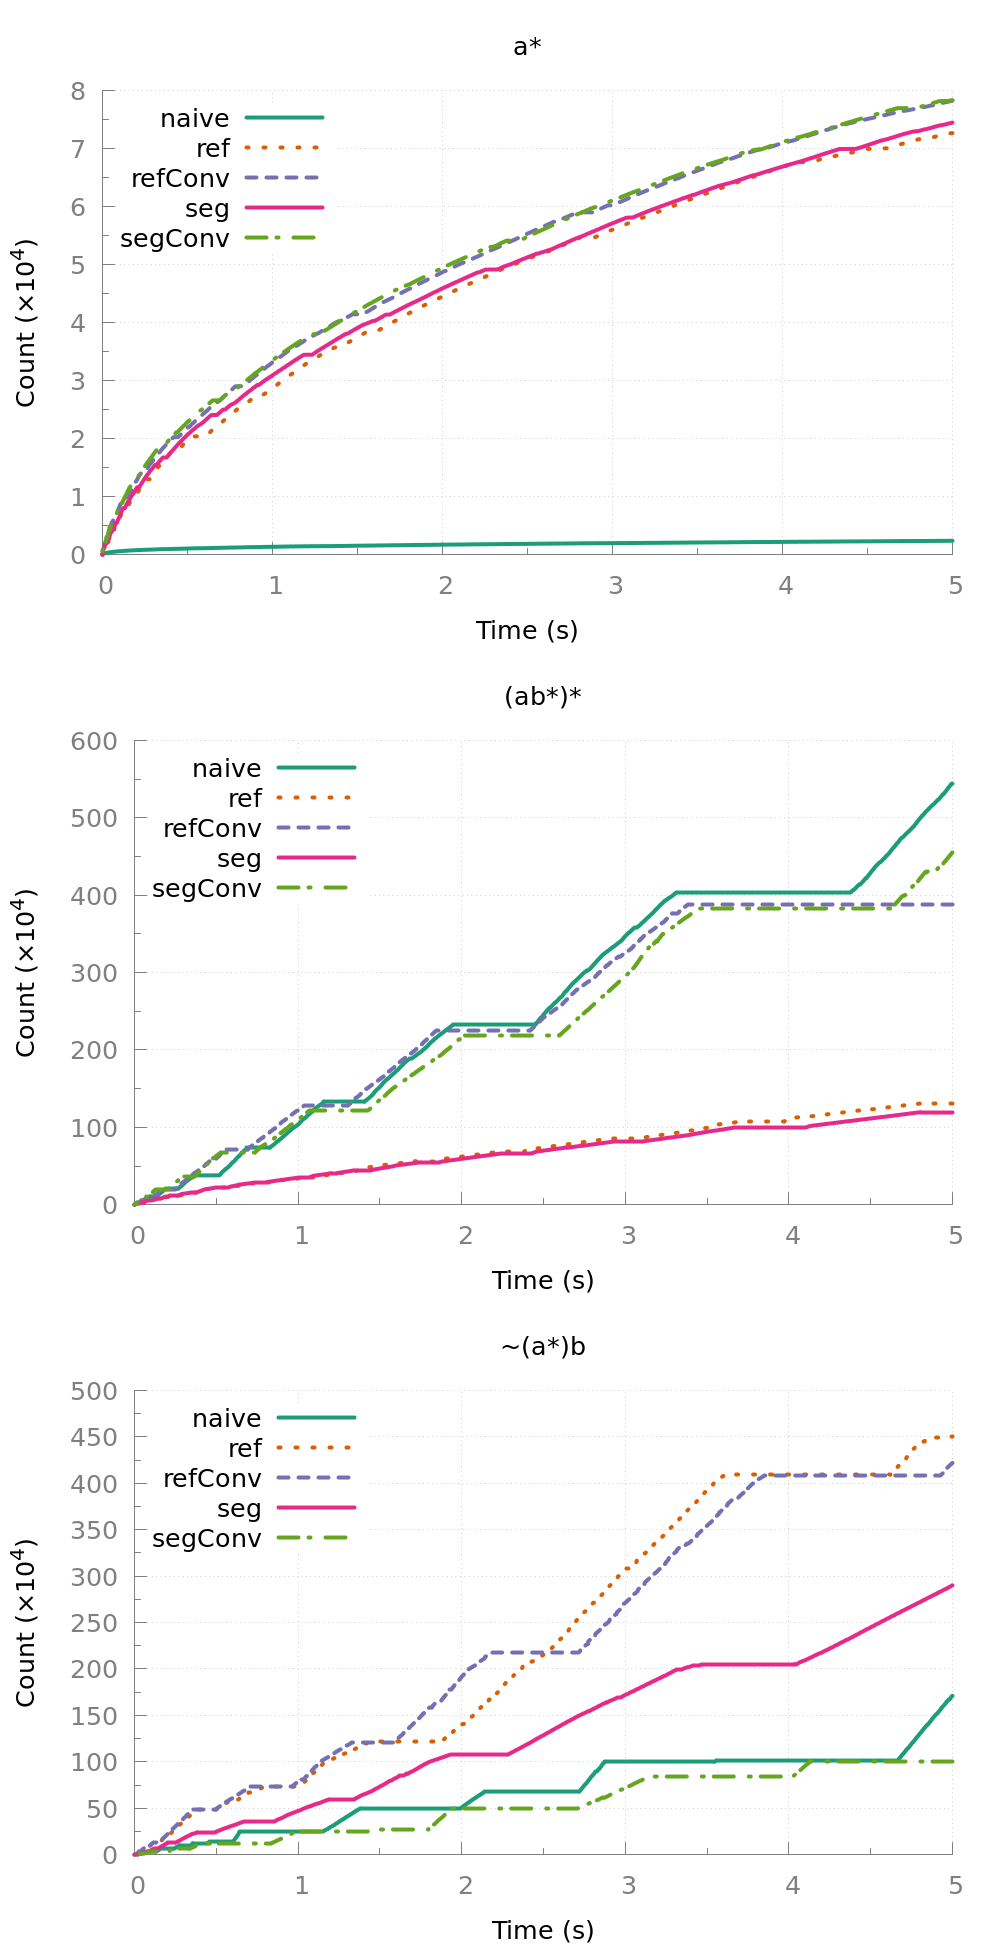
\includegraphics[height=0.33\linewidth]{measure/haskell_all.png}
  \caption{Benchmark for the \haskell implementation with various algorithms}
  \label{bench:haskell:all}
\end{figure}
To evaluate the performance, we iterate through the stream of words
produced by the generator and force their evaluation.\footnote{In
  Haskell, forcing is done using \lstinline{Control.DeepSeq}.} Every
20 words, we record the time elapsed since the start of the iteration. We
stop the iteration after 5 seconds. The resulting graph plots the time (x-axis) against the number of words (y-axis) produced so far. The slope of the graph in indicates the generation speed of the plotted algorithm, high slope is correlated to high generation speed.  \cref{bench:haskell:all} contains the results for the Haskell implementations.

Most algorithms generate between 3000 and
150000 words in the first second, which seems more than sufficient for
testing purposes.  Additionally, the refConv implementation which uses
symbolic segments and convolutions is the most versatile. This observation
validates that the changes proposed in \cref{sec:improvements} actually lead to improvements.

Looking at each graph in more detail, we can make the following
remarks:
\begin{itemize}[leftmargin=*]
\item All implementations are equally fast on $\Rstar a$ except
  the naive implementation, which  relies on list lookups without
  sparse indexing.
\item For $\Rstar{(\Rconcat{a}{\Rstar{b}})}$ and
  $\Rconcat{\Rcomplement{(\Rstar{a})}}{b}$, the graph of some implementations
  has the shape of ``skewed stairs''. We believe this phenomenon is due to
  insufficient laziness: when arriving at a new segment, part of the
  work is done eagerly which causes a plateau. When that part is done,
  the enumeration proceeds lazily.  As laziness and GHC
  optimizations are hard to control, we did not attempt to correct this.
\item $\Rstar{(\Rconcat{a}{\Rstar{b}})}$ demonstrates that sparse indexing
  does degrade performance when applying \code{star} to non-sparse languages.
  Using the convolution technique presented in \cref{sec:convolution} resolves this problem.
\item The \textbf{ref} and \textbf{refConv} algorithms are
  significantly faster on $\Rconcat{\Rcomplement{(\Rstar{a})}}{b}$
  compared to \textbf{seg} and \textbf{segConv}. We have no good
  explanation for this behavior as the code is identical up to the
  symbolic representation of full and empty segments. However, the
  only sublanguage where this representation could make a difference
  is $\Lang{b}$, which is also represented finitely by
  \textbf{segConv} and should thus benefit from the convolution
  improvement in the same way as \textbf{refConv}.
\end{itemize}


\subsection{Comparing data-structures in the \ocaml implementation}
\label{sec:bench:ocaml}

We have now established that the refConv algorithm provides the best performances.
The \haskell implementation, however, only uses lazy lists. To measure
the influence of strictness and data-structure on language generation,
we turn to the functorized \ocaml implementation.
We follow the same methodology than the \haskell evaluation using
the regular expressions
$\Rstar a$, $\Rstar{(\Rconcat{a}{\Rstar{b}})}$ and
$\Rconcat{\Rcomplement{(\Rstar{a})}}{b}$.
The results are shown in \cref{bench:ocaml:all}.

\begin{figure}[b]
  \centering
  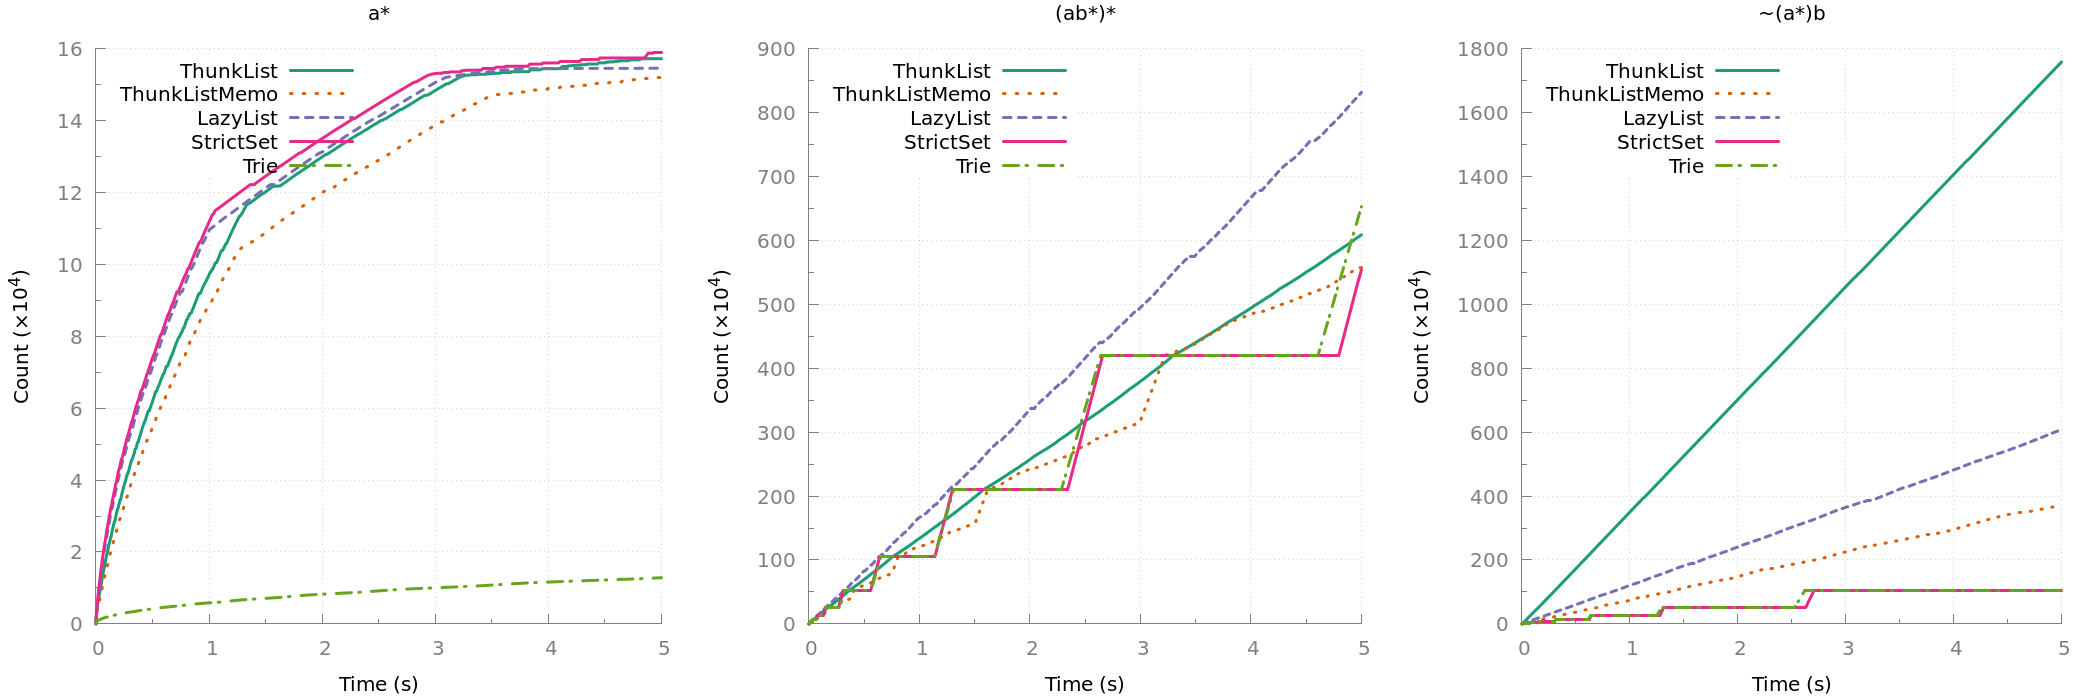
\includegraphics[height=0.33\linewidth]{measure/ocaml_all.png}
  \caption{Benchmark for the \ocaml implementation with various data-structures}
  \label{bench:ocaml:all}
  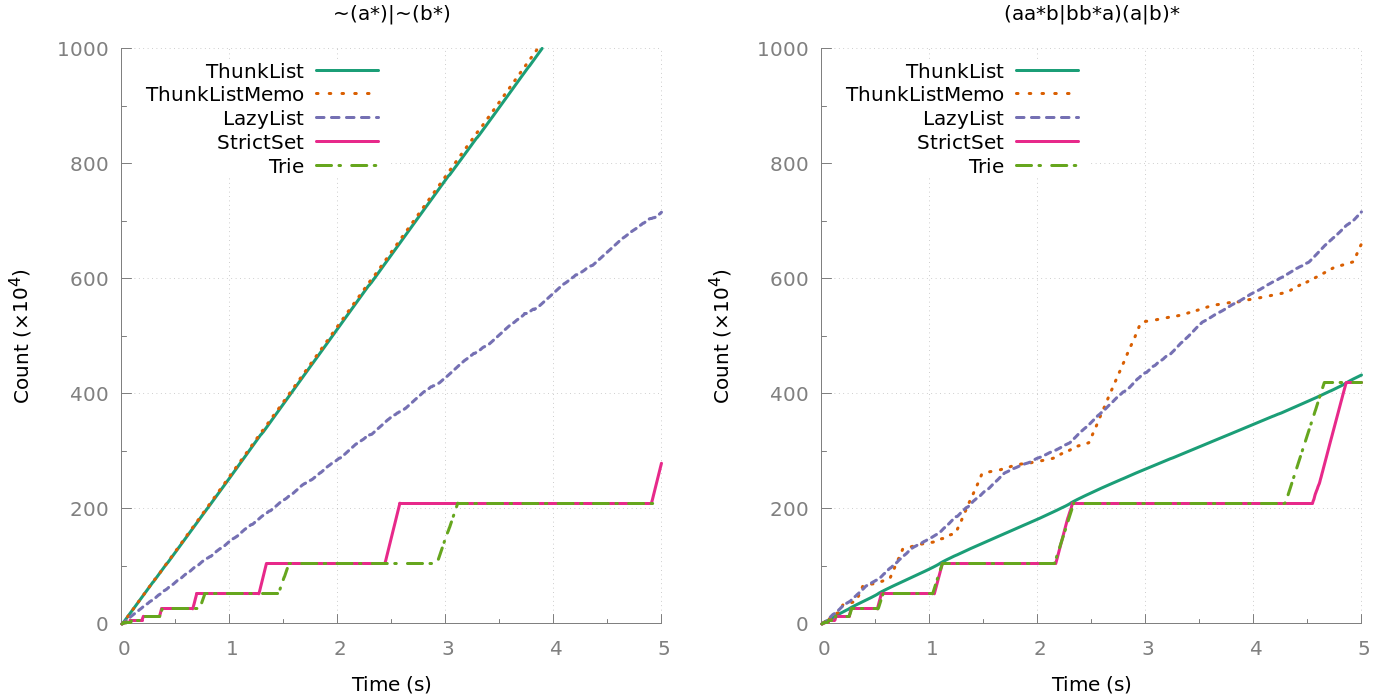
\includegraphics[height=0.33\linewidth]{measure/ocaml_union.png}
  \caption{Benchmarking \texttt{union} in the \ocaml data-structures}
  \label{bench:ocaml:union}
\end{figure}

Unlike the previous benchmark for algorithms, there is no clearly winner
among data-structures. The \code{ThunkList} and \code{LazyList} modules seem to
be superior to the alternatives, although the result are highly influenced by
the regular expression considered:
\begin{itemize}[leftmargin=*]
\item The \code{Trie} module is very inefficient on $\Rstar a$. Unfortunately,
  our implementation of tries doesn't use path compression. Each
  branch is only labeled by a single character.
  In the case of $\Rstar a$, each segment contains only one word and the
  trie degenerates to a list of character.
  We believe
  an implementation of tries with path compressions would perform similarly to
  the other data-structures.
\item The other data-structures on $\Rstar a$ exhibit a very pronounced slowdown
  when reaching 150000 words.
  We believe this is due to garbage collection: indeed
  all data-structure were consuming up to 10Go of memory before
  a collection was triggered. Memory consumption for the other regular
  expressions was far less significant.
\item Strict data-structure showcase a very marked ``skewed stair'' pattern.
  This pattern is however completely absent for \code{ThunkList} and
  \code{LazyList}. This demonstrates, if that was still needed,
  that laziness does indeed work very well in \ocaml. These results also confirm
  that strict data-structures should only be used when one wants to obtain
  all the elements up to a given length, in which case the stair pattern
  doesn't cause any penalty.
\item Memoization for thunk lists significantly decreases performances. It seems
  that the linear cost of memoizing the thunk list and allocating the vectors
  is higher than simple recomputing lists.
\end{itemize}

While the regular expressions presented previously do exercise
\code{concatenation} and \code{star}, they do not exercise set operations.
In order to test set operations on non-trivial segments (segments that
are neither full nor empty), we consider the language of words with at least
one $a$ and one $b$. This language can be built in two ways:
$\Runion{\Rcomplement{\Rstar{a}}}{\Rcomplement{\Rstar{b}}}$ and
$\Rconcat{(\Runion{a\Rstar{a}b}{b\Rstar{b}a})}{\Rstar{\Sigma}}$.
The first applies \code{union} to two large languages, the second takes
the union of smaller languages, but uses a concatenation.
The performances of the various data-structure on these two regular expressions
are presented in \cref{bench:ocaml:union}.
Lazy and thunk lists, with memoization or not, are very efficient on the union of languages but less so when concatenation is involved. Performance of strict sets and tries is surprisingly poor.

\subsection{The influence of regular expressions on performances}

As we have seen on the various benchmarks, the performance of the language
generator highly depends on the precise structure of both
the generated language and the regular expression considered.
We attempt to explore this remark by comparing various regular expressions
with the \code{refConv} \haskell implementation and the \code{ThunkList}
\ocaml implementation.
Before presenting the results, a word of warning:
We do not claim to offer a fair comparison between languages!
The two implementations are not exactly the same and we made no attempt
to measure both language in exactly the same conditions.
The comparison is shown in \cref{bench:langs}. In order to better visualize the
various regular expressions, the word count uses a logarithmic scale.

In addition to the regular expressions presented previously, we added the following:
\begin{itemize}
\item $\Rstar{(\Sigma\Sigma)}$, the language of words of lenght pair. This language
  is neither finite nor cofinite and make great use of the symbolic
  representation of segments.
\item $\Rstar{(\Runion{1 \Rstar{(0\Rstar{1}0)}1}{0})}$, the language
  of multiple of 3 written in binary. Again, this is a language that is neither
  finite nor cofinite, but its segments are never full nor empty.
\item $\Rstar{a}b$ and $b\Rstar{a}$, which allow us to see if
  \code{concatenation} has symmetric performances.
\end{itemize}

We remark that languages are roughly ordered by size. It is faster
to generate a language whose segments are bigger. Indeed,
most of the operations, notably
those involving product of segments, are more expansive when considering
segments of higher indices, thus making longer strings harder to generate.
If each segment contain many words, we do not need to compute many segments to
generate a large number of words.
%
We also note that the generation of $\Rstar{a}b$ and $b\Rstar{a}$
has indeed the same performance in the \haskell implementation.
The \ocaml version is however asymmetric, since it does not implement
the improved convolution technique with
detection of finite languages, as described in \cref{sec:convolution}.


\begin{figure}[h]
  \centering
  \begin{subfigure}[t]{0.45\linewidth}
    \centering
    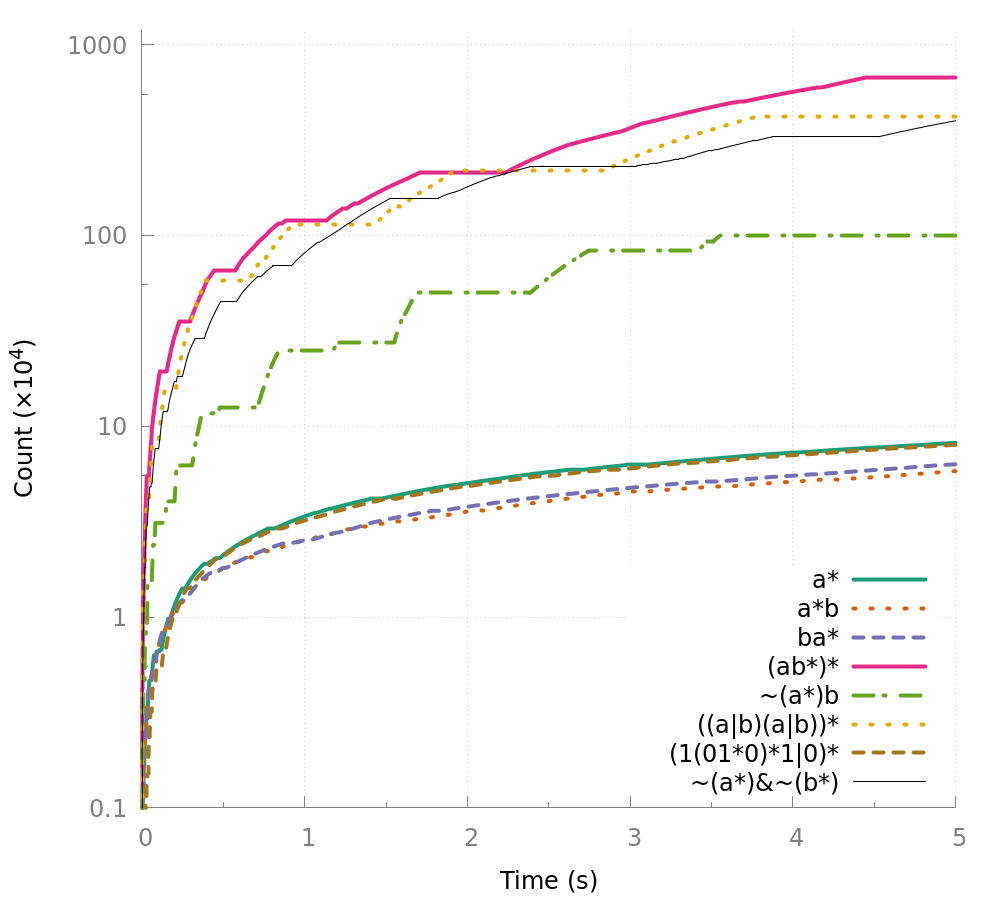
\includegraphics[width=\linewidth]{measure/haskell_langs.png}
    \caption{\haskell implementation with \code{segConv}}
    \label{bench:haskell:langs}
  \end{subfigure}
  \begin{subfigure}[t]{0.45\linewidth}
    \centering
    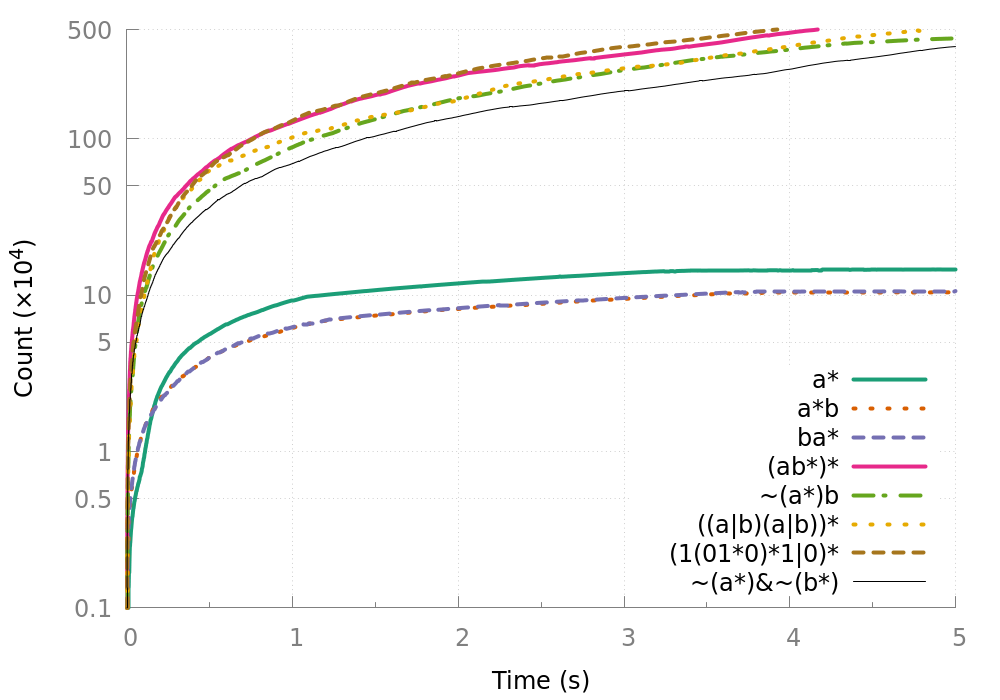
\includegraphics[width=\linewidth]{measure/ocaml_langs.png}
    \caption{\ocaml implementation with \code{ThunkList}}
    \label{bench:ocaml:langs}
  \end{subfigure}
  \caption{Benchmark on different regular expressions}
  \label{bench:langs}
\end{figure}

%%% Local Variables:
%%% mode: latex
%%% TeX-master: "main"
%%% End:
